% Tightness: point masses walking off the line, and one compact holding a family.
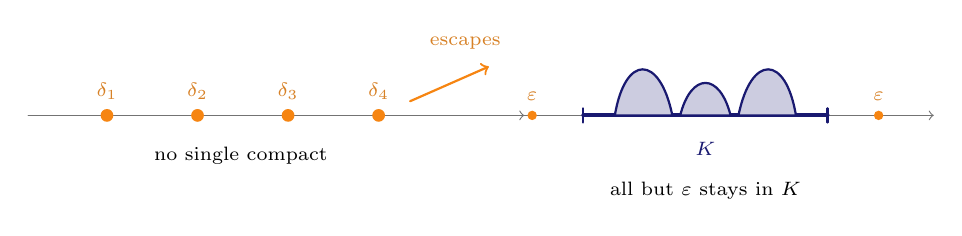
\begin{tikzpicture}[x=1cm,y=1cm,line cap=round,line join=round]
  \draw[black!55,->] (0,0) -- (6.3,0);
  \fill[BurntOrange] (1.0,0) circle (2.3pt);
  \fill[BurntOrange] (2.15,0) circle (2.3pt);
  \fill[BurntOrange] (3.3,0) circle (2.3pt);
  \fill[BurntOrange] (4.45,0) circle (2.3pt);
  \node[font=\scriptsize,BurntOrange!85!black,above] at (1.0,0.08) {$\delta_1$};
  \node[font=\scriptsize,BurntOrange!85!black,above] at (2.15,0.08) {$\delta_2$};
  \node[font=\scriptsize,BurntOrange!85!black,above] at (3.3,0.08) {$\delta_3$};
  \node[font=\scriptsize,BurntOrange!85!black,above] at (4.45,0.08) {$\delta_4$};
  \draw[BurntOrange,thick,->] (4.85,0.18) -- (5.85,0.62);
  \node[font=\scriptsize,BurntOrange!85!black] at (5.55,0.92) {escapes};
  \node[font=\scriptsize,below] at (2.7,-0.28) {no single compact};

  \begin{scope}[xshift=8.6cm]
    \draw[black!55,->] (-2.7,0) -- (2.9,0);
    \draw[MidnightBlue,line width=1.5pt] (-1.55,0) -- (1.55,0);
    \draw[MidnightBlue,thick] (-1.55,-0.09) -- (-1.55,0.09);
    \draw[MidnightBlue,thick] (1.55,-0.09) -- (1.55,0.09);
    \draw[MidnightBlue,thick,fill=MidnightBlue!22]
      (-1.15,0) .. controls (-1.02,0.78) and (-0.58,0.78) .. (-0.42,0) -- cycle;
    \draw[MidnightBlue,thick,fill=MidnightBlue!22]
      (-0.32,0) .. controls (-0.18,0.55) and (0.18,0.55) .. (0.32,0) -- cycle;
    \draw[MidnightBlue,thick,fill=MidnightBlue!22]
      (0.42,0) .. controls (0.58,0.78) and (1.02,0.78) .. (1.15,0) -- cycle;
    \fill[BurntOrange] (-2.2,0) circle (1.7pt);
    \fill[BurntOrange] (2.2,0) circle (1.7pt);
    \node[font=\scriptsize,BurntOrange!85!black,above] at (-2.2,0.06) {$\varepsilon$};
    \node[font=\scriptsize,BurntOrange!85!black,above] at (2.2,0.06) {$\varepsilon$};
    \node[font=\scriptsize,MidnightBlue,below] at (0,-0.22) {$K$};
    \node[font=\scriptsize,below] at (0,-0.72) {all but $\varepsilon$ stays in $K$};
  \end{scope}
\end{tikzpicture}
